%----------------------------------------------------------------------------------------
%	PACKAGES AND THEMES
%----------------------------------------------------------------------------------------
\documentclass[aspectratio=169,xcolor=dvipsnames]{beamer}
\usetheme{Simple}

\usepackage{hyperref}
\usepackage{graphicx} % Allows including images
\usepackage{booktabs} % Allows the use of \toprule, \midrule and \bottomrule in tables
\usepackage{mathtools}
\usepackage{amssymb}
\usepackage{graphicx}
\usepackage{ragged2e}
\usepackage{hyperref}
\hypersetup{
    colorlinks=true,
    linkcolor=black,
    urlcolor=blue,
}


%----------------------------------------------------------------------------------------
%	TITLE PAGE
%----------------------------------------------------------------------------------------

% The title
\title[short title]{Insumos de estimación}
\subtitle{Algoritmos}

\author[Nicolás Rivera] {Nicolás Rivera Garzón}
\institute[UNAL] % Your institution may be shorthand to save space
{
    % Your institution for the title page
    Departamento de Estadística \\
    Universidad Nacional de Colombia 
    \vskip 3pt
}
\date{Abril, 2021} % Date, can be changed to a custom date


%----------------------------------------------------------------------------------------
%	PRESENTATION SLIDES
%----------------------------------------------------------------------------------------

\begin{document}

% Portada: personalización arriba
\begin{frame}
    \titlepage
\end{frame}

% Tabla de contenidos
\begin{frame}{Contenido}
    \tableofcontents
\end{frame}


%------------------------------------------------
    % Primera Sección: Problemas de Algoritmo: MLE
    \section{Problemas Algorítmicos: MLE}
%------------------------------------------------

\begin{frame}{Problemas Algorítmicos: MLE}
    \begin{itemize}
        \item \justifying{Las estimaciones de máxima verosimilitud pueden no estar dadas explícitamente por fórmulas, sino implícitamente como soluciones de sistemas de ecuaciones no lineales.}
        \item \justifying{En el modelo de regresión clásico con matriz de diseño de rango completo, la fórmula del parámetro es fácil de escribir simbólicamente pero no es fácil de evaluar si el rango es grande.}
    \end{itemize}   
    \begin{block}{Modelo de regresión lineal simple (múltiple)}
       \justifying{Para los datos ${(z_{i},Y_{i};i=1,\dots,n)}$, el modelo en forma matricial es:} 
        $$Y=Z_{D}\beta+\epsilon$$
       \justifying{donde $Z_{D}$ es la matriz de diseño. La parametrización es identificable si y solo si $Z_{D}$ es de rango \textit{d} o de manera equivalente, si $Z_{D}^{t}Z_{D}$ es de rango completo \textit{d}. En ese caso la solución es:} 
       $$\hat\beta=[Z_{D}^{t}Z_{D}]^{-1}Z_{D}^{t}Y$$
    \end{block}
\end{frame}

%------------------------------------------------

%------------------------------------------------
    % Segunda Sección: Bisection
    \section{Método de Bisección}
%------------------------------------------------

\begin{frame}{Método de Bisección}
\justifying{Si la verosimilitud es diferenciable y la ubicación del máximo global está en el interior del espacio de parámetros, encontrar la solución se reduce a encontrar el resultado de las ecuaciones normales de verosimilitud. Los pasos del método son} 
    \begin{enumerate}
        \item \justifying{Encontrar dos puntos, uno en el que la derivada está por debajo de cero y otro que está por encima.}
        \item \justifying{Tomar la mitad del intervalo formado por estos puntos y cortarlo a la mitad.}
        \item Evaluar el valor de la derivada en el medio y reemplazar  por el punto medio uno de los puntos originales que tiene el mismo signo del valor de la derivada.
        \item \justifying{Continuar hasta que la longitud del intervalo tenga la precisión deseada o se alcance el cero antes de eso.}
    \end{enumerate}
\end{frame}

\begin{frame}{Bisección: Pseudocódigo}
\justifying{Dada una función continua \textit{f} en $(a,b)$, \textit{f} estrictamente creciente y $f(a+)<0<f(-b)$, entonces el \textbf{teorema del valor intermedio} garantiza que existe  una única $x^{*}\in (a,b)$ tal que $f(x^{*})=0$. Con esto en mente, el método de bisección encuentra $x^{*}$ con el pseudocódigo:}
    \begin{enumerate}
        \item \justifying{Encontrar $x_{0}<x_{1},f(x_{0})<0<f(x_{1})$, tomando $|x_0|,|x_1|$ suficientemente grandes, iniciar el algoritmo con $x_{old}^{+}=x_{1}, x_{old}^{-}=x_{0}$}
        \item \justifying{Si $|x_{old}^{+}-x_{old}^{-}|<2\epsilon$, entonces $x_{final}=\frac{1}{2}(x_{old}^{+}+x_{old}^{-})$ y declarar $x_{final}$}
        \item \justifying{De otro modo, $x_{new}=\frac{1}{2}(x_{old}^{+}+x_{old}^{-})$}
        \item \justifying{Si $f(x_{new})=0$, entonces, $x_{final}=x_{new}$ y declarar $x_{final}$}
        \item \justifying{Si $f(x_{new})<0$, entonces, $x_{old}^{-}=x_{new}$}
        \item \justifying{Si $f(x_{new})>0$, entonces, $x_{old}^{+}=x_{new}$}
        \item \justifying{Volver al paso 2}
    \end{enumerate}
\justifying{El algoritmo de bisección para en la solución $x_{final}$ tal que:
        $$|x_{final}-x^{*}|\leq \epsilon$$}
\end{frame}

\begin{frame}{Bisección para la familia exponencial uniparamétrica}
    \begin{block}{Teorema 2.4.1}        
    \justifying{Sea $p(x,\eta) $ una familia exponencial canónica de un parámetro generada por $(T,H)$, entonces, el estimador $\hat{\eta}$ de máxima verosimilitud se puede encontrar (con tolerancia $\epsilon$) por el método de bisección aplicado a:
    $$f(\eta)\equiv E_{\eta}T(X)-t_{0}$$ }\end{block}
    \begin{itemize}
        \item \justifying{Para la familia gamma de parámetro de forma con $X_1, \dots , X_n$ i.i.d. $\Gamma(\theta,1)$ de la forma:
        $$p(x;\theta)=\Gamma^-1(\theta)x^{\theta-1}e^{-x},x>0,\theta>0$$
        Ya que $T(X)=\sum^{n}_{i=0}log(X_i)$ tiene una densidad para todo $n$ tal que el estimador de máxima verosimilitud existe. De esta forma, se tiene que solucionar la ecuación: 
        $$\frac{\Gamma^{'}(\theta)}{\Gamma(\theta)}=\frac{T(X)}{n}$$
        que se puede evaluar por el método de bisección por el teorema anterior.}
    \end{itemize}
\end{frame}

%------------------------------------------------

%------------------------------------------------
    % Tercera Sección: Algoritmo de Escalada
    \section{Algoritmo de ascenso por coordenadas}
%------------------------------------------------

\begin{frame}{Algoritmo de ascenso por coordenadas: extensión a parámetros multidimensionales}
\justifying{El problema a considerar es resolver numéricamente, para la familia exponencial canónica de $k$ parámetros, la ecuación normal de:
$$E_{\eta}(T(X))=\Dot{A}=t_{0}$$
donde el estimador de máxima verosimilitud de $\hat{\eta}\equiv \hat{\eta}(t_0)$ existe. Aunque el algoritmo sea lento, siempre converge a $\hat{\eta}$. \bigskip

El método de ascenso por coordenadas es el algoritmo de bisección aplicado
a cada coordenada en forma iterativa de reciclaje.}
\end{frame}

\begin{frame}{Ascenso por coordenadas: Pseudocódigo}
\justifying{Para encontrar $\hat{\eta}$ se siguen los siguientes pasos:} 
\begin{enumerate}
    \item \justifying{Comenzar con un $\hat{\eta}^{0}=(\hat{\eta}^{0}_{1}, \dots, \hat{\eta}^{0}_{k})$ arbitrario, preferiblemente con una estimación ad hoc.}
    \item \justifying{Resolver las ecuaciones para las primeras derivadas de la forma:} 
    \begin{align*}
        \hat{\eta}^{1}_{1}&:\frac{\partial}{\partial\eta_{1}}A(\eta_{1}, \hat{\eta}^{0}_{2},\dots,\hat{\eta}^{0}_{k})=t_1\\
        \hat{\eta}^{1}_{2}&:\frac{\partial}{\partial\eta_{2}}A(\hat{\eta}^{1}_{1},\eta_2, \hat{\eta}^{0}_{3},\dots,\hat{\eta}^{0}_{k})=t_2\\
        \hat{\eta}^{1}_{k}&:\frac{\partial}{\partial\eta_{k}}A(\hat{\eta}^{1}_{k}, \hat{\eta}^{1}_{2},\dots,\hat{\eta}^{0}_{k})=t_k
    \end{align*}
\item \justifying{Definir $\hat{\eta}^{01}\equiv(\hat{\eta}^{1}_{1},\hat{\eta}^{0}_{2}, \dots, \hat{\eta}^{0}_{k}), \hat{\eta}^{02}\equiv(\hat{\eta}^{1}_{1},\hat{\eta}^{1}_{2}, \hat{\eta}^{0}_{3},\dots, \hat{\eta}^{0}_{k})$ y sucesivamente.}
\item \justifying{Repetir el proceso hasta eventualmente encontrar $\hat{\eta}^{(r)}$ con una tolerancia igual a:}  $$|\hat{\eta}^{jl}-\hat{\eta}^{j(l-1)}|\leq \epsilon$$
\end{enumerate}
\end{frame}

\begin{frame}{¿Por qué funciona?}
    \begin{columns}[t] 
        \column{.55\textwidth} 
        \begin{itemize}
            \item \justifying{La log-verosimilitud es cóncava.}
            \item \justifying{El algoritmo encuentra el máximo a lo largo de una de las coordenadas, mientras que todas las demás se fijan de modo que el valor de la verosimilitud aumenta en cada paso del algoritmo.}
            \item \justifying{La log-verosimilitud está limitada en el interior del conjunto de  parámetros, por lo que tiene que haber un límite.}
            \item \justifying{Gracias a ello, $\hat{\eta}^{(r)}$ debe estar en una bola cerrada en el interior del espacio de parámetros.} 
        \end{itemize}
        \column{.45\textwidth} 
        \begin{figure}
            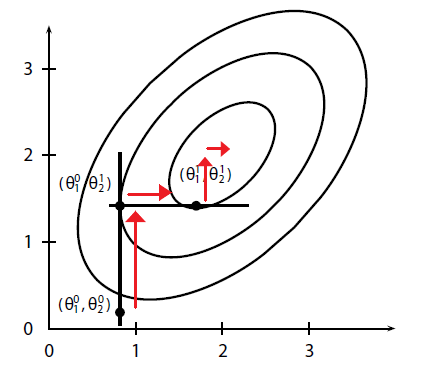
\includegraphics[width=1\linewidth]{Ascent.PNG}
        \end{figure}
    \end{columns}
\end{frame}

%------------------------------------------------

%------------------------------------------------
    % Cuarta Sección: Algoritmo Newton-Raphson
    \section{Algoritmo Newton-Raphson}
%------------------------------------------------

\begin{frame}{Algoritmo Newton-Raphson}
    \begin{itemize}
        \item \justifying{Este método requiere el cálculo de la inversa de la hessiana, lo que puede contrarrestar su ventaja en la velocidad de convergencia sobre el ascenso por coordenadas, cuando converge.}
         \item \justifying{La lógica de su pseudocódigo es sencilla, si $\hat{\eta}_{old}$ es el valor actual del algoritmo entonces:}
                $$\hat{\eta}_{new}=\hat{\eta}_{old}-\ddot{A}^{-1}(\Dot{A}(\hat{\eta}_{old})-t_0)$$
        \justifying{Si $\hat{\eta}_{old}$ está cerca de la raíz $\hat{\eta}$ de $\Dot{A}(\hat{\eta})=t_0$, entonces por la expansión de $\Dot{A}(\hat{\eta})$ alrededor de $\hat{\eta}_{old}$ se obtiene:}
$$t_{0}-\Dot{A}(\hat{\eta}_{old})=\Dot{A}(\hat{\eta})-\Dot{A}(\hat{\eta}_{old})\simeq \ddot{A}(\hat{\eta}_{old})(\hat{\eta}-\hat{\eta}_{old})$$
$\hat{\eta}_{new}$ es la solución para la aproximación dada por la ecuación. El algoritmo tiene la propiedad que para $n$ grande, $\hat{\eta}_{new}$ se comporta aproximadamente como MLE después de un paso. 
    \end{itemize}
\end{frame}

\begin{frame}{Newton-Raphson para MLE y familia exponencial}
\begin{itemize}
    \item Para una función de log-verosimilitud $l(\theta)$:
    $$\hat{\theta}_{new}=\hat{\theta}_{old}-\ddot{l}_{-1}(\hat{\theta}_{old})\dot{l}(\hat{\theta}_{old})$$
    \item Para una familia exponencial canónica: 
    $$\hat{\eta}_{new}=\hat{\eta}_{old}-\ddot{A}^{-1}(\hat{\eta}_{old})(\dot{A}(\hat{\eta}_{old})-t_0)$$
\end{itemize}
Cuando las probabilidades no son cóncavas, se siguen empleando métodos como bisección, ascenso coordinado y Newton-Raphson.
Existe una clara posibilidad de no convergencia o convergencia a un máximo local en lugar de global.
\end{frame}


%------------------------------------------------

%------------------------------------------------
    % Quinta Sección: Algoritmo esperanza-maximización
    \section{Algoritmo esperanza-maximización (EM)}
%------------------------------------------------

\begin{frame}{Algoritmo esperanza-maximización (EM): Motivación}
Existen muchos modelos que tienen la siguiente estructura:  
    \begin{itemize}
        \item \justifying{Hay observaciones ideales, $X\sim P(\theta)$ con densidad $p(x;\theta), \theta \in \Theta \subset R^{d}$.}
        \item \justifying{Su función de log-verosimilitud $l_{p,x}(\theta)$ es fácil de maximizar.}
        \item \justifying{Sin embargo, se observan datos incompletos dados por $S\equiv S(X) \sim Q_{\theta}$ con densidad $q(s,\theta)$ donde $l_{q,s}(\theta)=log(q(s,\theta))$ es difícil de maximizar. Su función no es cóncava y es compleja de computar,}
        \item \justifying{Una forma de pensar en tales problemas es en términos de $S$ como datos incompletos y que representan una parte de $X$, y su "reconstrucción" es parte del proceso de estimación por máxima verosimilitud de $\theta$.}
    \end{itemize}
\end{frame}

\begin{frame}{Algoritmo EM}
\begin{enumerate}
    \item Iniciar con $\theta_{old}=\theta_0$
    \item Sea:
    $$J(\theta|\theta_0)\equiv E_{\theta_{0}}(\log \frac{p(X,\theta)}{p(X,\theta_0}|S(X)=S)$$
    \item Paso E: evaluar $J(\theta|\theta_0)$ para tantos valores de $\theta$ como sea necesario.
    \item Paso M: Maximizar $J(\theta|\theta_0)$ como una función de $\theta$.
    \item Definir $\theta_{new}=\arg \max J(\theta|\theta_0)$
    y reiniciar $\theta_{old}=\theta_{new}$ y repetir el proceso. 
\end{enumerate}
\begin{block}{Lema 2.4.1}
Si $\theta_{new}$,$\theta_{old}$ se definen como en el pseudocódigo y $S(X)=s$ entonces: 
$$q(s,\theta_{new}) \geq q(s,\theta_{new})$$
La igualdad se cumple si la la distribución condicional de $X$ dada $S(X)=s$ es la misma para $\theta_{new}$ como $\theta_{old}$ y $\theta_{old}$ maximiza $J(\theta|\theta_{old})$
\end{block}
\end{frame}

\begin{frame}{EM para familias exponenciales}
\begin{block}{Teorema 2.4.3}
Sea $P_{\theta}:\theta \in \Theta$ una familia exponencial canónica generada por $(T,h)$ y sea $S(X)$ cualquier estadístico, entonces: 
\begin{enumerate}
    \item El algoritmo EM consiste de la alternancia de:
    $$\dot{A}(\theta_{new})=E_{\theta_{old}}(T(X)|S(X)=s)$$
    $$\theta_{old}=\theta_{new}$$
    \item Si:
    $$\dot{A}(\theta)=E_{\theta}(T(X)|S(X)=s)$$
    tiene una única solución que converge a $\hat{\theta^{*}}$ que es necesariamente un máximo local de $q(s,\theta)$.
    \end{enumerate}
\end{block}
\end{frame}

\begin{frame}{Referencias}
\begin{itemize}
    \item Bickel, P., & Doksum, K. (2015). Mathematical statistics. Boca Raton: CRC Press.
    \item El repositorio con la presentación y las simulaciones se encuentra en \href{https://github.com/nriverag/Insumos-de-estimacion}{GitHub}.
\end{itemize}
\end{frame}

%------------------------------------------------
\end{document}